\chapter{Saddle point approximation}
\label{cha:sp_approx}

%A semi-classical analysis of ATI which describes the formation of the
%ionization spectrum based on the interference of quantum paths is
%included in Sec.~\ref{sec:spa}. The direct ionization regime is
%considered independently in Sec.~\ref{sec:spa_direct}. The analysis
%presented in this chapter closely follows that
%of~\cite{KopoldOptComm2000}.

%\section{\label{sec:spa} Saddle point approximation}

For laser fields of sufficiently high intensity, the \textsc{ati}
spectrum can be generated by implementing a saddle point
evaluation~\cite{LewensteinSPA_1994} of the multidimensional integral
for the transition amplitude obtained in the previous chapter. This
semi-classical approximation provides a deeper physical insight than
the expansion in Bessel functions from the improved Keldysh
approximation~\cite{Kopold_1997sfa}, as it captures the essential
underlying physics. It also establishes a connection between
\textsc{ati} calculations within the framework of the strong-field
approximation and the concept of quantum
paths~\cite{KopoldOptComm2000}, which represent space-time
trajectories of the tunneling electrons. This concept has its origins
in the alternative formulation of quantum mechanics introduced by
Feynman in terms of path integrals~\cite{RevModPhysFeynman}, in which
the probability amplitude of a quantum mechanical process can be
represented as a coherent superposition of contributions from all
possible spatio-temporal paths that connect the initial and final
state of the system.

This chapter presents the arguments of Kopold
et. al.~\cite{KopoldOptComm2000,phd_Kopold} in an attempt to reproduce
their study of \textsc{ati} with electron rescattering on atoms and
test for numerical stability. In view of this, the arguments
introduced in their saddle-point analysis of \textsc{ati} are
presented in the following sections. The saddle-point approximation
establishes the connection between the quantum mechanical path
integral formalism and the improved Keldysh approximation discussed in
Sec.~\ref{kopold_sfa}. The transition amplitude that describes the
ionization of an electron under an external laser field is evaluated
within the two frameworks, that in which only direct electrons are
considered as well as the case that incorporates rescattering off the
parent ion. Our study follows those in Refs.~\cite{Kopold_1997sfa,
  KopoldOptComm2000}.

% see pra51 lewenstein

% mention that now that the matrix element for ionization has been
% introduced in the previous chapter, we are going to discuss an
% approximation to obtain the ionization spectrum where the integral
% over time is solved based on the stationary points method

\section{\label{sec:q_paths} Quantum-orbit formalism}

Several quantum models have been introduced in the literature that
extend the scope of the Keldysh approximation for strong laser-atom
interactions. A generalization of the Keldysh-Faisal-Reiss
(\textsc{kfr}) formulation of \textsc{ati} explores the dynamics of
the ionized electrons under a high-intensity laser, including
rescattering effects, by means of a representation of the
time-evolution operator as an expansion with respect to the
interaction with the atomic binding
potential~\cite{Kopold_1997sfa}. The \textsc{kfr} theory of
strong-field approximation has also been extended to the study of
harmonic generation~\cite{LewensteinSPA_1994,Lewenstein_1995} by means
of a quantum model that takes into account additional interaction of
the ionizing electron with the ion core including higher order terms
in a perturbative expansion leading to rescattering effects. This
model, non restricted to zero-range potentials, constitutes a quantum
mechanical formulation of the two-step semiclassical
picture~\cite{Becker_2step1986}, which has proven to be crucial in
understanding strong-field laser-atom interactions. These models,
which incorporate rescattering effects of the excited electrons, have
been valuable in unraveling the physical phenomena behind the
\textsc{ati} plateau and its cutoff, an intrinsic feature of the
ionization spectrum.

A quasi-classical analysis of this generalization, based on the
saddle-point method and the path integral
formalism~\cite{KopoldOptComm2000,Becker_ellipticalSPA,LewScience2001},
has been particularly useful as it illustrates fundamental aspects of
the physics underlying strong-field ionization processes as well as
the formation of their spectra. This approach suggests that one
pictures the processes taking place in laser-atom interactions, such
as \textsc{ati} and high-harmonic generation (\textsc{hhg}), in terms
of electron trajectories in phase space. These quantum trajectories,
as it is explained below, follow classical Newtonian dynamics,
however, must take place in the complex plane to account for tunneling
ionization. Consequently, they present non-zero imaginary components
which determine the probability of the process. Their physical content
is reflected in the electron dynamics once it has been ionized at time
$t'$, the electron may return to its parent ion at a later time $t$
and rescatter after propagating with momentum $\mathbf{k}$ in the
continuum under the action of the external field.

As a starting point in the evaluation of the \textsc{ati} probability
amplitude~\ref{eq:mp_compact} by means of a saddle-point approximation
we consider the compact form of the Volkov state in the length gauge
(see Appendix~\ref{app:L_gauge}), which can be expressed
as~\cite{Becker_ati2002}
%
\begin{eqnarray}
\label{eq:volkov_Lgauge}
\begin{split}
|\psi_{\mathbf{p}}^{(V)}(t)\rangle & = &
|\mathbf{p} - e\mathbf{A}(t)\rangle e^{-i S_{\mathbf{p}}(t)},
\end{split}
\end{eqnarray}
%
where $|\mathbf{p} - e\mathbf{A}(t)\rangle$ represents a plane-wave
state with momentum $\mathbf{k} = \mathbf{p} - \mathbf{A}(t)$ and
$S_{\mathbf{p}}(t) = 1/2m \int\limits^{t} d\tau [\mathbf{p} -
  e\mathbf{A}(\tau)]^{2}$ denotes the action of the system. The Volkov
time-evolution operator, which replaces the exact time-evolution
operator in the strong-field approximation~\cite{KeldyshSFA},
satisfies the Schr\"{o}dinger equation
%
\begin{eqnarray}
  \label{eq:Uv_SchEq}
  \begin{split}
    [ i\partial_{t} - H_{I}(t) ] U^{(V)}(t,t') = 0 \\
    H_{L}(t) = -\frac{1}{2}\nabla^{2} + V_{I}(t)
  \end{split}
\end{eqnarray}
%
where $V_{I}(t) = \mathbf{r}\cdot\mathbf{E}(t)$ indicates the
interaction of the electron with the electric field of the laser. It
can be verified that the Volkov time-evolution operator, expressed in
terms of a Volkov-state decomposition~(\ref{eq:volkov_Lgauge}) by
%
\begin{eqnarray}
\label{eq:te_volkov}
\begin{split}
U^{(V)}(t,t') & = & \int d^{3}\mathbf{k}
|\psi_{\mathbf{k}}^{(V)}(t) \rangle
\langle \psi_{\mathbf{k}}^{(V)}(t')|,
\end{split}
\end{eqnarray}
%
is the solution to the initial-value problem~(\ref{eq:Uv_SchEq}), with
$U^{(V)}(t',t') = \hat{1}$, where $\hat{1}$ is the unit operator, in
view of the completeness of the plane-wave states as required by the
evolution operators formalism~\cite{BeckerTEOp_2006,cjp2010_keldysh}.
%(seeJPhysB39)

Inserting the expansion~(\ref{eq:te_volkov}) into the matrix
element~(\ref{eq:mp_compact}) and taking into acount the time
dependence of the ground state wave function, $|\psi_{0}(t) \rangle =
\exp{(iE_{0}t)} | \psi_{0} \rangle$, one may write the probability
amplitude as the five-dimensional integral~\cite{KopoldOptComm2000}
%
\begin{eqnarray}
  \label{eq:mp_5Dintegral}
  \begin{split}
    M_{\mathbf{p}} \sim & \int\limits_{-\infty}\limits^{\infty} dt
    \int\limits_{-\infty}\limits^{t} \int d^{3}\mathbf{k}\ 
    \langle [\mathbf{p} - e\mathbf{A}(t)] e^{iS_{\mathbf{p}}(t)} | V |
    \mathbf{k} - e\mathbf{A}(t) \rangle e^{-iS_{\mathbf{k}}(t)} \\
    & \times
    \langle [\mathbf{k} - e\mathbf{A}(t')] e^{iS_{\mathbf{k}}(t')} | V |
    \psi_{0} \rangle e^{iE_{0}t'} \\
    \sim &
    \int\limits_{-\infty}\limits^{\infty} dt
    \int\limits_{-\infty}\limits^{t} \int d^{3}\mathbf{k}\ 
    \exp\ i\left[ S_{\mathbf{p}}(t) - S_{\mathbf{k}}(t)
      + S_{\mathbf{k}}(t') + E_{0}t' \right] \\
    & \times
    \langle \mathbf{p} - e\mathbf{A}(t) | V |
    \mathbf{k} - e\mathbf{A}(t) \rangle 
    \langle \mathbf{k} - e\mathbf{A}(t') | V |
    \psi_{0} \rangle.
  \end{split}
\end{eqnarray}
%
The action for \textsc{ati}, in the exponent
of~(\ref{eq:mp_5Dintegral}) consists of three terms
%
\begin{eqnarray}
  \label{eq:action_mpintegral}
  \begin{split}
    S_{\mathbf{p}}(t, t', \mathbf{k}) & = & - \frac{1}{2m}
    \int\limits_{t}\limits^{\infty} d\tau [\mathbf{p} - e\mathbf{A}(\tau)]^{2}
    - \frac{1}{2m} \int\limits_{t'}\limits^{t} d\tau [\mathbf{k} - e\mathbf{A}(\tau)]^{2}
    + \int\limits_{-\infty}\limits^{t'} d\tau E_{0},
  \end{split}
\end{eqnarray}
%
which correspond to the action of the entire system after rescattering
at time $t$, between ionization and rescattering where the
intermediate free-electron momenta is indicated by $\mathbf{k}$, and
before the electron is ionized at time $t'$, respectively. The
rescattering amplitude, $M_{\mathbf{p}}$, which accounts for the
high-energy plateau in the electron energy spectrum, takes the
form~\cite{Becker_ati2002,BeckerTEOp_2006}
%
\begin{eqnarray}
\label{eq:mp_final}
\begin{split}
M_{\mathbf{p}} \sim &
\int\limits_{-\infty}\limits^{\infty} dt
\int\limits_{-\infty}\limits^{t} dt'
\int d^{3}\mathbf{k} \exp \left[ iS_{\mathbf{p}}(t, t', \mathbf{k}) \right]
m_{\mathbf{p}}(t, t', \mathbf{k}),
\end{split}
\end{eqnarray}
%
with
%
\begin{eqnarray}
  \label{eq:mp_braketfunction}
  \begin{split}
    m_{\mathbf{p}}(t, t', \mathbf{k}) & = &
    \langle \mathbf{p} - e\mathbf{A}(t) | V |
    \mathbf{k} - e\mathbf{A}(t) \rangle 
    \langle \mathbf{k} - e\mathbf{A}(t') | V |
    \psi_{0} \rangle.
  \end{split}
\end{eqnarray}
%
This amplitude corresponds to the so-called three-step
model~\cite{Becker_ati2002}, in which $V$ represents the potential
that the ionized electron feels when it rescatters off its parent
ion. In order to evaluate the total probability amplitude, one needs
to integrate over the interval of ionization times $t'$ during which
the electric field is non-zero, integrate over all intermediate
electron momenta $\mathbf{k}$, and over all rescattering times $t >
t'$. The amplitude~(\ref{eq:mp_final}) can be approximated using a
saddle-point method~\cite{Lewenstein_1995}, in which the leading
contribution to the \textsc{ati} spectrum is determined by requiring
stationarity of the quasiclassical
action~(\ref{eq:action_mpintegral}).
% comment from JphysB39 about evaluating Mp using a saddle-point
% approximation


% point out the contrast with feynman's path integral
% p-57 chapter
It is revealing to point out the contrast of the ionization
amplitude~(\ref{eq:mp_final}), obtained with the strong-field
approximation, with its analogous representation in terms of Feynman's
path integral formulation~\cite{RevModPhysFeynman}. The time evolution
operator of the entire system has the path integral representation
\begin{eqnarray}
\label{eq:te_path}
\begin{split}
U(\mathbf{r}t, \mathbf{r}'t') & = &
\int\limits_{(\mathbf{r}',t')\to(\mathbf{r},t)}
\mathcal{D}\left[ \mathbf{r}(\tau) \right] e^{i S(t, t')},
\end{split}
\end{eqnarray}
where $S(t, t') = \int\limits_{t'}\limits^{t} d\tau
\mathcal{L}[\mathbf{r}(\tau), \tau]$ is the action calculated along a
specific path by integrating the Lagrangian of the entire system along
that path, and the integral measure denoted by $\mathcal{D}\left[
  \mathbf{r}(\tau) \right]$ establishes a coherent sum over all
possible paths that connect $(\mathbf{r}t)$ and $(\mathbf{r}'t')$,
independently of whether or not the paths might be followed by the
actual system. This sum is, in fact, an infinite-dimensional
functional of integrals, and can be reduced, within the framework of
the strong-field approximation, to a sum over a few quantum orbits. By
implementing the strong-field approximation we have approximated the
exact action of the system at the various stages of the process:
before ionization, in between ionization and rescattering, and after
rescattering, as Eq.~(\ref{eq:action_mpintegral}) indicates. The
ionization amplitude is then computed by means of a sum over the
exponential of the action over a five-parameter set of paths,
parametrized by the ionization time $t'$, the rescattering time $t$
and the canonical momentum of the orbit denoted by
$\mathbf{k}$~\cite{KopoldOptComm2000}.

% ref from Principles...Lewenstein&LHuillier
% it is needed here an explanation of what the saddle-point
% approximation is and why it is justified to use it
In the low-frequency limit and for high-intensity laser fields, the
five-dimensional set of paths over which the transition
amplitude~(\ref{eq:mp_final}) is evaluated can be reduced further by
invoking the saddle-point approximation~\cite{,Lewenstein_1995} to
calculate the integral over $\mathbf{p}$ as well as $t$ and $t'$. In
this regime, the transition amplitude contains a rapidly oscillating
factor, $\exp\ iS_{\mathbf{p}}(t, t', \mathbf{k})$, provided that the
parameters $U_{p}$, $I_{p}$, and $p^{2}$ in the quasi-classical
action~(\ref{eq:action_mpintegral}) are large enough. The major
contributions to the integrals in~(\ref{eq:mp_final}) come from the
saddle points, which are the solutions of $S''_{\mathbf{p}}(q_{i}) =
0$ that render the phase stationary.
% mention deformation of the integration path into the complex plane
% mention why the trajectories are complex
In the process of evaluating the transition amplitude, the phase of
the integrand is expanded about the saddle-points along the path of
steepest descent in the complex plane. As a result, a handful of
relevant paths remains to be considered in order to explore the
\textsc{ati} spectrum~\cite{KopoldOptComm2000}. Since the tunneling
process of an electron is involved in this analysis, these paths take
place in the complex plane.
%
The condition
\begin{eqnarray}
\label{eq:S_stationary}
\begin{split}
\frac{\partial S}{\partial q_{i}} & = & 0
\end{split}
\end{eqnarray}
where $q_{i}(i =1, \dots, 5)$ runs over the five variables $t$, $t'$
and $\mathbf{k}$, leads to the saddle-point
equations~\cite{Lewenstein_1995,KopoldOptComm2000}
\begin{eqnarray}
\label{eq:saddle_eqs}
\begin{split}
\left( \mathbf{k} - e\mathbf{A}(t') \right)^{2} = &
-2m|E_{0}| \\
\left( \mathbf{k} - e\mathbf{A}(t)\right)^{2} = &
\left( \mathbf{p} - e\mathbf{A}(t) \right)^{2} \\
(t - t') \mathbf{k} = & \int\limits_{t'}\limits^{t}
d\tau e\mathbf{A}(\tau).
\end{split}
\end{eqnarray}
The solutions $(t_{S}(\mathrm{Re}\ t_{S} > \mathrm{Re}\ t'_{S}),
t'_{S}, \mathbf{k}_{S})$, are known as the stationary points of the
quasicassical action of the system, and define the quantum orbits
which are the essential components in building the ionization spectrum
through the saddle-point approximation. From a physical perspective,
Eqs.~(\ref{eq:saddle_eqs}) ensure the energy conservation at the time
of tunneling, elastic scattering of the electron into its final state
when it returns, and that in fact the electron returns to its parent
ion, respectively. Since $|E_{0}| > 0$ in~(\ref{eq:saddle_eqs}), the
condition of energy conservation at the time of ionization cannot be
satisfied for any real time $t'$. As a consequence, the solutions
$(t_{S}, t'_{S}, \mathbf{k}_{S})$ of the saddle-point equations
describe complex orbits which restrains a straightforward
visualization of the trajectories.

%p-56 chapter ATI
The probability amplitude~(\ref{eq:mp_final}) can now be expressed in
terms of the saddle-point solutions as~\cite{KopoldOptComm2000}
\begin{eqnarray}
\label{eq:Mp_final}
\begin{split}
M_{\mathbf{p}} \sim & \sum\limits_{i} \left( \frac{(2\pi i \hbar)^{5}}
{\mathrm{det} (\partial^{2}S / \partial q_{j} \partial q_{k})_{j,k = 1, \dots, 5}}
\right)^{1/2} \times \exp(i S(t_{S_{i}}, t'_{S_{i}}, \mathbf{k}_{S_{i}})),
\end{split}
\end{eqnarray}
where $q_{i}(i = 1,\dots,5)$ runs over the five variables $t_{S},
t_{S}'$ and $\mathbf{k}_{S}$. The sum~(\ref{eq:Mp_final}) involves a
reduced set of trajectories that are sufficient to approximate the
ionization spectrum through their interferences, which have
constructive and destrutive contributions.


\section{\label{sec:spa_results} Results}
% mention that we explore the quantum trajecotries that are relevant
% to the ATI spectrum

This section presents the results corresponding to a saddle-point
analysis of the probability amplitude to detect \textsc{ati} electrons
that emerge from a model-helium atom under a strong laser field of the
form~(\ref{eq:lp_field}). In order to obtain comparable results to the
quantum generalization of the strong-field approximation presented in
Chapter~\ref{cha:ati}, the laser intensity and frequency were set to
$I = 10^{15}\ \mathrm{W/cm^{2}}$ and $\hbar\omega =
0.0584\ \mathrm{a.u.}$, respectively.

% introduce direct trajectories and rescattering

\subsection{\label{sec:spa_direct} Direct trajectories}

The probability amplitude for detecting an \textsc{ati} electron that
propagates with momentum $\mathbf{p}$ in the continuum as a result of
the laser irradiation of an atom, originally in its ground state, is
studied in this section. The action of a system consisting of a bound
electron that is ionized at time $t_{0}$, without further interaction
with the parent ion, has the form~\cite{phd_Kopold,Becker_ati2002}
%
\begin{eqnarray}
  \label{eq:action_direct}
  \begin{split}
  S_{\mathbf{p}}(t_{0}) & = &
-\frac{1}{2m}\int_{t_{0}}^{\infty}{d\tau [\mathbf{p} - e\mathbf{A}(\tau)]^{2}}
- \int_{-\infty}^{t_{0}}{d\tau E_{0}},
\end{split}
\end{eqnarray}
%
where $\mathbf{A}(t)$ represents the vector potential of the laser
field, and $E_{0}$ is the binding energy of the atom. As the main
contribution to the transition amplitude~(\ref{eq:Mp_final}) is given
by the stationary points of the action which satisfy the condition
$dS_{\mathbf{p}} / dt_{0} = 0$, the integral~(\ref{eq:Mp_final}) is
evaluated by implementing a saddle-point
approximation~\cite{spa_1960}. This consists in expanding the phase of
the integrand, $\Phi(t) = (1/\eta) S(t) = (\omega / U_{p}) S(t)$, in
the vicinity of the points where the phase is stationary, which
results in determining the solutions of
%
\begin{eqnarray}
  \label{eq:stationary_points}
  \begin{split}
    \frac{\partial S_{\mathbf{p}}}{\partial t_{0}} & = &
    \frac{1}{2m} (\mathbf{p} - e\mathbf{A}(t_{0}))^{2} + |E_{0}| = 0.
  \end{split}
\end{eqnarray}
%
The stationary points from Eq.~(\ref{eq:stationary_points}) have a
non-zero imaginary component, therefore, it is convenient to split the
integral of the action~(\ref{eq:action_direct}) into the complex plane
by implementing the substitution $\omega t_{0} \to \rm{Re}(\omega
t_{0}) + i\rm{Im}(\omega t_{0})$. For a linearly polarized laser field
of the form~(\ref{eq:lp_field}), the location of the saddle points can
be determined analytically and their real and imaginary components
satisfy the conditions
%
\begin{eqnarray}
  \label{eq:ReIm_eqs}
  \begin{split}
    \cos^{2}(\rm{Re}\ \omega t_{0s}) = & \frac{1}{2}
    \left( 1 + \gamma^{2} + \frac{E_{p}}{2U_{p}} \right)
    - \frac{1}{2}\sqrt{\left( \frac{E_{p}}{2U_{p}} \right)^{2}
    + (1 + \gamma^2)^2 + \frac{E_{p}}{U_{p}}(\gamma^2 - \cos 2\phi)}
    \\
    \cosh(\rm{Im}\ \omega t_{0s}) = & - \sqrt{\frac{E_{p}}{2U_{p}}}
    \frac{\cos\phi}{\cos(\rm{Re}\ \omega t_{0s})},
  \end{split}
\end{eqnarray}
%
where $m = -e = 1$, and $\phi$ is the angle between the momentum
$\mathbf{p}$ and the direction of polarization of the laser field,
$\hat{x}$. The electron energy, as it propagates in the continuum, is
indicated by $E_{p} = p^{2}/2m$. As Eqs.~(\ref{eq:ReIm_eqs}) indicate,
a single electron energy $E_{p}$ is associated with four saddle-points
$\omega t_{0s}$, $s = 1, \dots, 4$, which are related to each other by
complex conjugation.  These complex roots are illustrated in
Figure~\ref{fig:sp_direct} for electron energies within the range $(0,
\dots, 6U_{p})$. The saddle points with positive imaginary parts,
$t_{01}$ and $t_{02}$, are shown in blue, whereas the red connected
dots, $t_{03}$ and $t_{04}$, indicate points with negative imaginary
parts. The contours defined by the saddle points in phase space
illustrate the integration paths to follow for a given electron energy
when constructing the \textsc{ati} spectrum.

% include plot with the saddle-points for direct trajectories
\begin{figure}
  \centering
  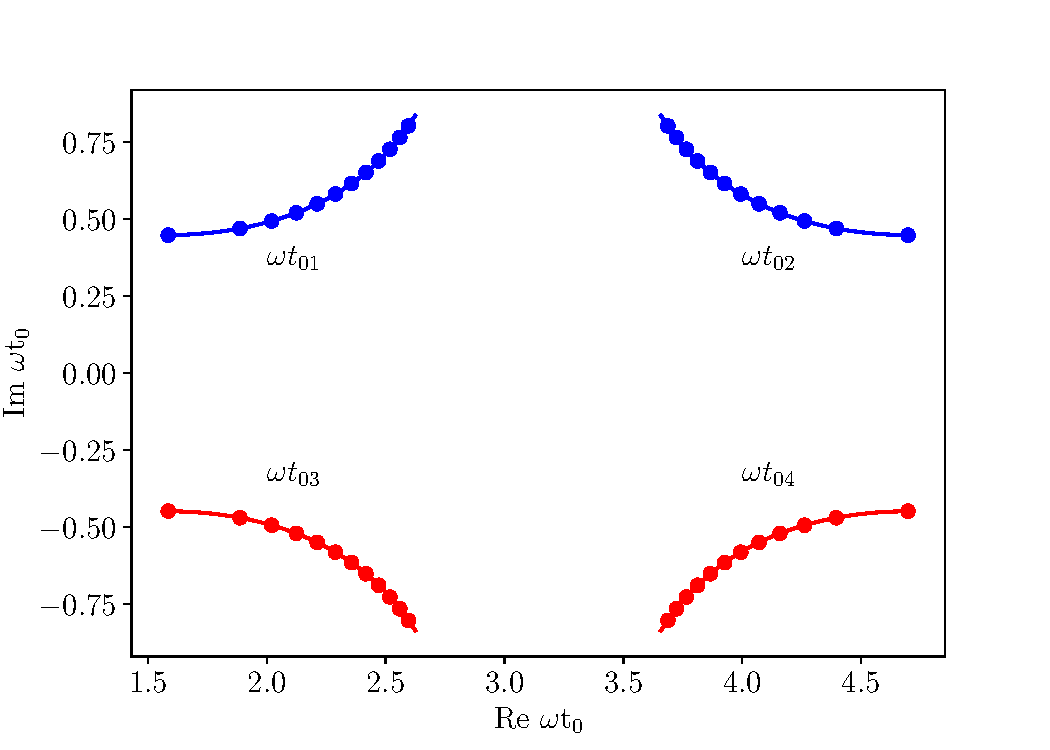
\includegraphics[width = 0.75\textwidth]{figures/ch_ATI_SPA/direct/spDirectElectrons}
  \caption{Representation of the saddle points corresponding to
    Eqs.~(\ref{eq:ReIm_eqs}) that indicate the complex ionization
    times associated with direct trajectories of electrons ionized by
    a linearly polarized field with laser intensity of
    $10^{15}\ \rm{W/cm^{2}}$ and $\hbar\omega = 1.58\ \rm{eV}$. The
    connected dots correspond to discrete energies within the range
    $(0, \dots, 6 U_{p})$. The trajectories with $\mathrm{Im}\ \omega
    t_{0i} > 0$ are shown in blue, while the ones with
    $\mathrm{Im}\ \omega t_{0i} < 0$ are indicated in red.}
  \label{fig:sp_direct}
\end{figure}

% - see Appendix B in Kopold dissertation where the Gaussian
% approximation is justified
% - explain what the method of steepest descend (or spa) consists of and
% how the integral defining the Mp vals can be expressed as a Gaussian
% as a result of this approximation
% - express Mp in eq.5.6 as a contour integral in terms of s(z) and g(z)
% as it is shown in appendix B of Kopold thesis
% - look up method of steepest descent.pdf
In a saddle-point evaluation of the integral~(\ref{eq:mp_final}), it
is convenient to refer to the assymptotic evaluation of the expression
%
\begin{eqnarray}
  \label{eq:I_eta_contour}
  I(\eta) = \int\limits_{\mathcal{C}} dz g(z) e^{\eta s(z)}
\end{eqnarray}
%
in the case where the functions $s(z)$ and $g(z)$ are analytic and
$\eta > 0$. The integration contour $\mathcal{C}$ is deformed into a
composition of contours $\mathcal{C}_{s}$ coinciding with the path of
steepest descent. This transformation into the complex plane, in which
the function $s(z = x + iy) = u(x,y) + iv(x, y)$, leads to express the
saddle-point condition as
\begin{eqnarray}
  \label{eq:sp_uv_complex}
  (\nabla u) \cdot (\nabla v) = 0,
\end{eqnarray}
% mention that the contour is chosen by method of steepest descent
% where Im(v) = constant and what that represents in terms of the
% saddle points contributions to the integral. then taylor expansion
% in the vicinity of the saddle points leads to the Gaussian function
% for Mp
indicating that the curves along the directions of $\nabla u$ and
$\nabla v$ always meet orthogonally at any point. Ideally, one needs a
path near a point $z = z_{s}$ such that $u(x,y)$ attains a peak and
decreases away from $z = z_{s}$. But the imaginary part $v(x,y)$ will
in general also change and the exponential factor $e^{i\eta v}$ will
oscillate rapidly in the vicinity of $z_{s}$. If the point $z = z_{s}$
coincides with a saddle point, a suitable path is one where $v(x,y)$
is nearly constant as one moves away from $z_{s}$, in other words,
when the exponential term in~(\ref{eq:I_eta_contour}) can be expressed
as
%
\begin{eqnarray}
  \label{eq:exp_steepest}
  e^{\eta u(x,y) + i \eta v(x,y)} = e^{\eta u(x,y)} e^{i \eta v(x_{s},y_{s})}.
\end{eqnarray}
%
Therefore, in order to calculate the saddle point contributions to the
integral, one chooses the integration path such that
$\mathrm{Im}\ s(z) = \mathrm{Im}\ s(z_{s})$. Along the direction of
steepest descent for the surface $u(x,y) = u(x_{s},y_{s})$, defined by
$-\nabla u|_{z_{s}}$, the Cauchy-Riemann equations justify that the
tangents to the surface $v(x,y) = v(x_{s},y_{s})$ lie in the direction
of steepest descent through $z_{s}$. In a contour $\mathcal{C}_{s}$
that goes through the saddle points of $s(z)$, the main contribution
to the integral in the transition probability comes from the saddle
point $z_{s} = x_{s} + iy_{s}$ or its immediate vicinity. Therefore, a
Taylor expansion of the action~(\ref{eq:action_direct}) around the
saddle point $z_{s}$ in the form
%
\begin{eqnarray}
  \label{eq:taylor_exp}
  s(z) \simeq s(z_{s}) + \frac{1}{2!}s''(z_{s})(z - z_{s})^{2} 
\end{eqnarray}
%
is justified. This approximation allows for an analytic determination
of the saddle point contributions to the
integral~(\ref{eq:I_eta_contour}), which can be written as a Gaussian
integral and evaluates to~\cite{phd_Kopold}
%
\begin{eqnarray}
  \label{eq:I_Gaussian}
  I(\eta) \simeq \sum\limits_{s\mathrm{\epsilon} \mathcal{Z}_{\mathcal{C}}}
  \pm g(z_{s}) e^{\eta s(z_{s})} \sqrt{\frac{2\pi}{-\eta s''(z_{s})}},
\end{eqnarray}
%
provided that the original contour $\mathcal{C}$ is deformed into a
composition $\mathcal{C}_{\mathrm{max}}$ of contours
$\mathcal{C}_{s,\mathrm{max}}$ which are regions where $s(z)$ and
$g(z)$ are analytic, with identical boundary points
$\partial\mathcal{C}_{\mathrm{max}} = \partial\mathcal{C}$. The sum
in~(\ref{eq:I_Gaussian}) runs over a partial set of all saddle points
whose contours $\mathcal{C}_{s,\mathrm{max}}$ combine into
$\mathcal{C}_{\mathrm{max}}$.

Accordingly, the \textsc{kfr} matrix element for direct electrons can
be approximated by a Gaussian function~\cite{phd_Kopold}
%
\begin{eqnarray}
  \label{eq:KFR_Mp}
  \begin{split}
    M_{\mathbf{p}} & \sim & \int\limits_{0}\limits^{T} dt\ e^{i \eta \Phi(t)},
  \end{split}
\end{eqnarray}
%
in which the phase is defined as $\Phi(t) = S_{\mathbf{p}}(t)\omega /
U_{p}$, and the period of the laser field is indicated by $T$. The
integration path to follow is defined by a contour of saddle points
whose locations, indicated in Eq.~(\ref{eq:ReIm_eqs}), are known
analitically for a linearly polarized laser field. This expression
results in~\cite{phd_Kopold}
%
\begin{eqnarray}
  \label{eq:Mp_spa_direct}
  \begin{split}
    M_{\mathbf{p}} & \sim & \sum\limits_{i}
    \sqrt{\frac{2\pi\hbar}{-i S''_{\mathbf{p}}(t_{s_{i}})}}
    \exp iS_{\mathbf{p}}(t_{s_{i}}),
  \end{split}
\end{eqnarray}
%
where $t_{s_{i}}$ denote the saddle points that lie in the contour of
interest. Equation~(\ref{eq:Mp_spa_direct}) approximates the
\textsc{ati} spectrum for an electron that, after being ionized at
some time $t_{0}$ under a strong laser field, propagates under the
influence of the field with no further interaction with the binding
potential.

% explain how to choose the relevant contours and the figure in phase space
% then explain eq.B25 from Kopold

In order to visualize the regions in phase space where the action
$S_{\mathbf{p}}$ is stationary and, consequently, construct an
integration path of stationary phase through the saddle-points, it is
convenient to carry out the substitution $t \to t_{r} + it_{i}$ in
Eq.~(\ref{eq:action_direct}). For a monochromatic laser
field~(\ref{eq:lp_field}), and assuming that the electron path is
parallel to the electric field of the laser, the real and imaginary
components of the phase take the form~\cite{phd_Kopold}
%
\begin{eqnarray}
  \label{eq:phase_im}
  \begin{split}
    \mathrm{Im}\ i\Phi(t) & = & \omega t_{r} ( 1 + \frac{E_{p}}{U_{p}}
    + 2\gamma^{2} ) +
    \frac{1}{2} \sin 2\omega t_{r} \cosh 2\omega t_{i}
    + 2\sqrt{\frac{2E_{p}}{U_{p}}} \sin\omega t_{r} \cosh\omega t_{i}
  \end{split}
\end{eqnarray}
%
\begin{eqnarray}
  \label{eq:phase_re}
  \begin{split}
    -\mathrm{Re}\ i\Phi(t) & = & \omega t_{i} (
    1 + \frac{E_{p}}{U_{p}} + 2\gamma^{2} )
    + \frac{1}{2} \cos 2\omega t_{r} \sinh 2\omega t_{i}
    + 2\sqrt{\frac{2E_{p}}{U_{p}}} \cos\omega t_{r} \sinh\omega t_{i}.
  \end{split}
\end{eqnarray}
%
At a given electron energy, the permited integration contours follow
from $\mathrm{Im}\ i \Phi(t) = \mathrm{Im}\ i \Phi(t_{si})$, and
Eq.~(\ref{eq:phase_im}) allows to write them explicitly as a function
of $t_{i}(t_{r})$. Figure~\ref{fig:sp_contours} shows contours for
constant imaginary part of the exponent in Eq.~(\ref{eq:KFR_Mp}), as
well as the set of saddle points corresponding to an electron energy
of $2.27 U_{p}$, indicated by crosses ($\times$). The blue curve
corresponds to contours with $\mathrm{Im}\ i \Phi(t) = \mathrm{Im}\ i
\Phi(t_{s_{1},s_{3}})$, while contours with $\mathrm{Im}\ i \Phi(t) =
\mathrm{Im}\ i \Phi(t_{s_{2},s_{4}})$ are indicated by a red
curve. The purple scale represents the real values of the exponent
$i\Phi(t)$, in which dark regions indicate small values of
$\mathrm{Re}\ i\Phi(t)$, while bright regions indicate large values of
$\mathrm{Re}\ i\Phi(t)$. This implies that, for every single electron
energy, $E_{p}$, only one possible integration path is relevant in
order to evaluate the transition amplitude $M_{\mathbf{p}}$. The one
starting at $t = 0$ to $+i\infty$, $C_{a}$, then along $C_{1}$ across
the saddle point $t_{01}$ up to $\omega t = \pi + i\infty$ where the
integrand vanishes, from there along $C_{2}$ across the second saddle
point, $t_{02}$, to $\omega t = 2\pi + i\infty$, and finally along
$C_{b}$ to $\omega t = 2\pi$. The integrands along $C_{a}$ and $C_{b}$
are identical and the integrals add up to zero due to the reversed
integration orders. Along contours $C_{1}$ and $C_{2}$, the integrand
is approximated by the Gaussian~(\ref{eq:Mp_spa_direct}) with $i = 1,
2$. For a given electron energy, $E_{p}$, the probability
amplitude~(\ref{eq:Mp_spa_direct}) is evaluated along the integration
trajectory that contains the saddle-points with positive imaginary
parts, $t_{01}$ and $t_{02}$, indicated as blue connected dots in
Figure~\ref{fig:sp_direct}, in order to obtain a converging result
when evaluating the exponential term in $M_{\mathbf{p}}$.
% add some reference to the path of steepest descent mentioned above
% to make this description connect with the formalism of saddle points

% include contour plots for constant values of Im(\Phi) and
% integration path
\begin{figure}
  \centering
  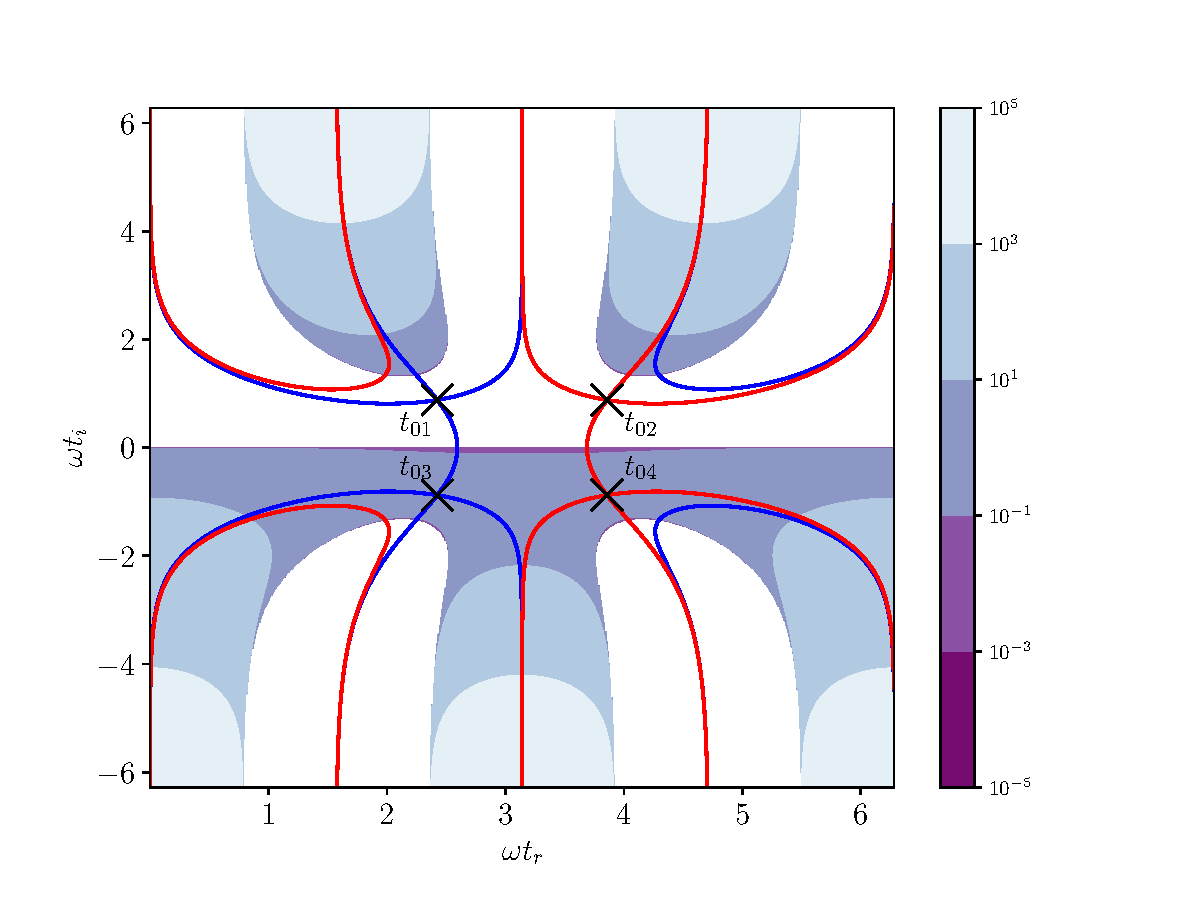
\includegraphics[width = 0.75\textwidth]{figures/ch_ATI_SPA/direct/phase_contour12}
  \caption{Phase contours of constant $\mathrm{Im}\ i\Phi(t)$ for the
    saddle points $t_{01}(t_{03})$ (blue lines) and $t_{02}(t_{04})$
    (red lines) corresponding to an electron energy of $2.27 U_{p}$
    projected on the complex plane. The allowed integration contour
    runs over the saddle points with positive imaginary parts,
    $t_{01}$ and $t_{02}$. The regions in a purple scale represent the
    real part of the exponent in Eq.~(\ref{eq:KFR_Mp}),
    $\mathrm{Re}\ i\Phi(t)$, in which dark/light regions stand for
    small/large real parts .}
  \label{fig:sp_contours}
\end{figure}

The described ionization spectrum of direct electrons for a model
helium atom calculated by means of the saddle-point
approximation~(\ref{eq:Mp_spa_direct}) is displayed in
Figure~\ref{fig:ati_direct} by dash-dotted lines. The \textsc{ati}
spectrum corresponding to the exact Keldysh amplitude is indicated
with black dots. The saddle-point approximation mirrors the fully
quantum calculation in terms of an expansion in Bessel
functions. Similarly to what the Keldysh \textsc{sfa} results point
out, the saddle-point approximation generates an \textsc{ati} spectrum
that vanishes at approximately $2.5 U_{p}$ as the electron escapes the
effects of the binding potential without further interaction with the
parent ion.

\begin{figure}
  \centering
  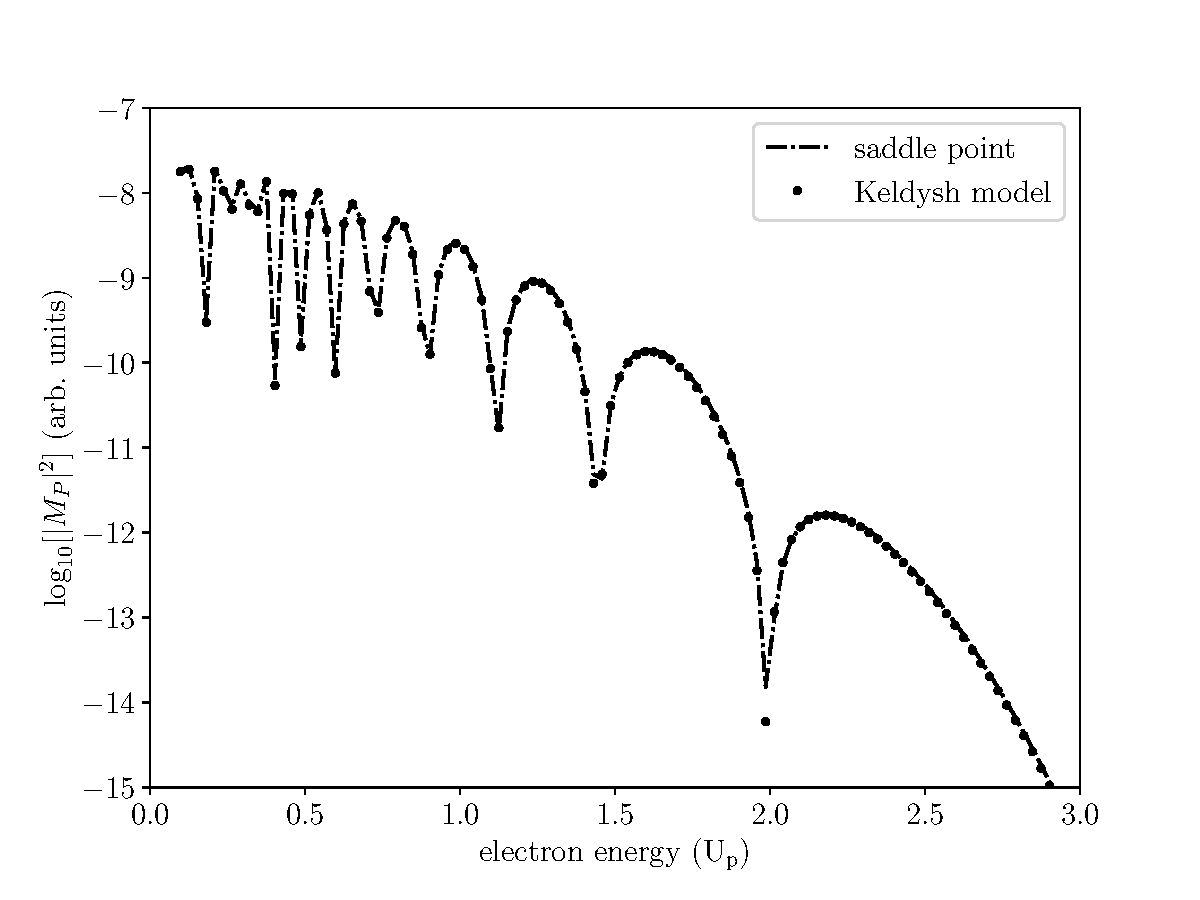
\includegraphics[width = 0.75\textwidth]{figures/ch_ATI_SPA/direct/SPvsKeldysh_spa_discrete}
  \caption{Calculated \textsc{ati} spectrum using Keldysh formalism
    (black dots) and the saddle-point approximation (dash-dot line) in
    terms of trajectories $1$ and $2$, for a laser intensity of
    $10^{15}\ \rm{W/cm^{2}}$, $\hbar\omega = 1.58\ \rm{eV}$, and a
    binding energy of $E_{0} = -0.9\ \rm{a.u.}$ for a zero-range He
    model. The electron energies are expressed in units of
    $U_{p}$. The Keldysh parameter was set to $\gamma = 0.654$, and
    the ratio $U_{p}/\omega$ was set to $\eta = 17.9$.}
  \label{fig:ati_direct}
\end{figure}


\subsection{\label{sec:spa_resc} Trajectories with rescattering}

% fundamental features of rescattering, how is this approached
% see PhysRevA55 comments about rescattering and the plateau (introduction)
Incorporating rescattering effects, in which ionized electrons are
allowed to return to the parent ion, is of great significance in the
study of \textsc{ati} as it expands the possible physical
interpretations to the ionization spectrum. In particular, it
elucidates the origin of the extended \textsc{ati} plateau which can
be observed at high electron energies~\cite{Walker_1996}. This
plateau, a key feature to the laser induced \textsc{ati}, is
thoroughly justified when rescattering effects are included in the
analysis~\cite{Paulus_1994plateau,BeckerRescattering_2018}, and has
been widely addressed in the literature under the hypothesis that the
electrons that are responsible for this plateau gain their energy
through backscattering when upon propagation in the laser field they
return to the vicinity of the parent
ion~\cite{Paulus_1994plateau,Becker_1994plateau_classical,Becker_rescattering1994}. It
is the purpose of this section to revisit a saddle-point approximation
of the rescattering picture in which the quantum orbits of the ionized
electron play an essential part in the formation of the \textsc{ati}
spectrum~\cite{KopoldOptComm2000}.


%has been well
%described by a three-step model that employs a zero-range binding
%potential as well as rescattering
%effects~\cite{Becker_rescattering1994,Kopold_1997sfa}. 


% equations to determine the physical magnitudes (t, t', k) that
% define the complex trajectories, i.e., saddle points
In the recollision picture, an electron transitions from the ground
state into the continuum at time $t'_{S}$, ionization time, from that
time on the effects of the laser field in the electron dynamics are
dominant and the Coulomb potential of the parent ion becomes
negligible as the electron propagates in the continuum with momentum
$\mathbf{k}_{S}$, however, the model accounts for further interaction
with the binding potential as the electron is considered to return to
within the vicinity of the ion at time $t_{S}$, rescattering time, at
which the electron acquires its final asymptotic momentum
$\mathbf{p}$.

The relevant quantum orbits, defined by the complex saddle points
$(t'_{S}, t_{S}, \mathbf{k}_{S})$, are the solutions of the
saddle-point equations~(\ref{eq:saddle_eqs}) which have their origin
in the condition that the action of the system remains stationary
along those points. For the linearly-polarized
field~(\ref{eq:lp_field}), after some algebraic work on the
saddle-point equations, one can solve for the rescattering time and
ionization time as the numerical solutions of~\cite{KopoldOptComm2000}
%
\begin{eqnarray}
  \label{eq:return_t}
  \begin{split}
    [\omega t_{S} \mp \arccos(2\cos\omega t_{S} + \delta \mp i\gamma)]
    (2\cos\omega t_{S} + \delta) \\
    \pm \sqrt{1 - (2\cos\omega t_{S} + \delta \mp i\gamma)^{2}} 
    - \sin\omega t_{S} = 0
  \end{split}
\end{eqnarray}
%
and
%
\begin{eqnarray}
  \label{eq:release_t}
  \begin{split}
    \omega t'_{S} = \mp \arccos(2\cos\omega t_{S} + \delta \mp i\gamma),
  \end{split}
\end{eqnarray}  
%
respectively, where the quantity $\delta$ is defined as $\delta =
\sqrt{p^{2} / (4mU_{p})}$. Therefore, the complex paths are generated
for every possible set of saddle points $(t'_{i}, t_{i},
\mathbf{k}_{i})$, where $i$ indicates the $i-$th quantum
trajectory. As Eq.~(\ref{eq:return_t}) indicates, solutions for the
rescattering time come in pairs for each optical cycle $T = 2\pi$ due
to the combination of $\pm$ signs. Additionally, the multivaluedness
of the $\arccos$ function leads to infinitely many
solutions. Considering the periodicity of the laser field, we can
focus our attention to the interval $0 < \mathrm{Re}\ t_{i} < T$ for
the rescattering times. Subsequently, Eq.~(\ref{eq:release_t})
produces two solutions for the ionization time within the interval
$-T/2 < \mathrm{Re}\ t'_{i} < 0$, two from the interval $-T <
\mathrm{Re}\ t'_{i} < -T/2$, and so forth. In
Figure~\ref{fig:orbit_pairs}, a subset of these numerical solutions
illustrates the described distribution for the release and return
times corresponding to the first six quantum orbits, $i = 1, \dots,
6$, for a fixed electron energy of $E_{p} = 6 U_{p}$.  The release
times (right panel) illustrate how additional pairs of solutions
become available for lower energies, with $t'_{i}$ extending further
into the past. The electric field of the laser, $\mathbf{E}(t) =
-\partial/\partial t \mathbf{A}(t)$, is depicted in the left panel
with dash-dotted lines for the optical cycle $0 < \omega t < T$ along
with the solutions for the return times.
 
The value of the ponderomotive energy, $U_{p}$, at which the two
trajectories of a given pair approach each other most closely
corresponds to the cutoff of this pair. Typically, the orbits that
correspond to a given cutoff energy are defined as long and short
orbit~\cite{BeckerRescattering_2018}. Each pair of trajectories
$(i,j)$ has its well defined cutoff at some energy,
$E_{\mathrm{cutoff}}$, at which the orbits come together, and the pair
ceases to contribute to the ionization spectrum for $E_{p} >
E_{\mathrm{cutoff}}$. The inset in the left panel of
Figure~\ref{fig:orbit_pairs} depicts the described behaviour for the
pair $(1,2)$ of quantum orbits, the curves indicate the numerical
solutions for the return times corresponding to three different values
of the electron energy. No solutions can be found for the return
times, and subsequently the release times, if the electron energy
exceeds the cutoff energy associated to a given pair. The cutoff
energy for the pair $(1,2)$ comes out to be $10.24 U_{p}$ as
Figure~\ref{fig:orbit_pairs} indicates. Typically, the travel time,
$\mathrm{Re}(t_{i} - t'_{i})$, associated to a quantum orbit indicates
the relevance of its contribution to the \textsc{ati} spectrum, the
ones with shorter travel time being qualitatively more relevant, as
they make up for the strongest contributions to the ionization
spectrum.
% include physical picture indicating that there are two solutions for
% each optical cycle, as it is mentioned in this paragraph

% include discussion of short and long trajectories following this
% paragraph
\begin{figure}
  \begin{subfigure}[b]{0.55\linewidth}
    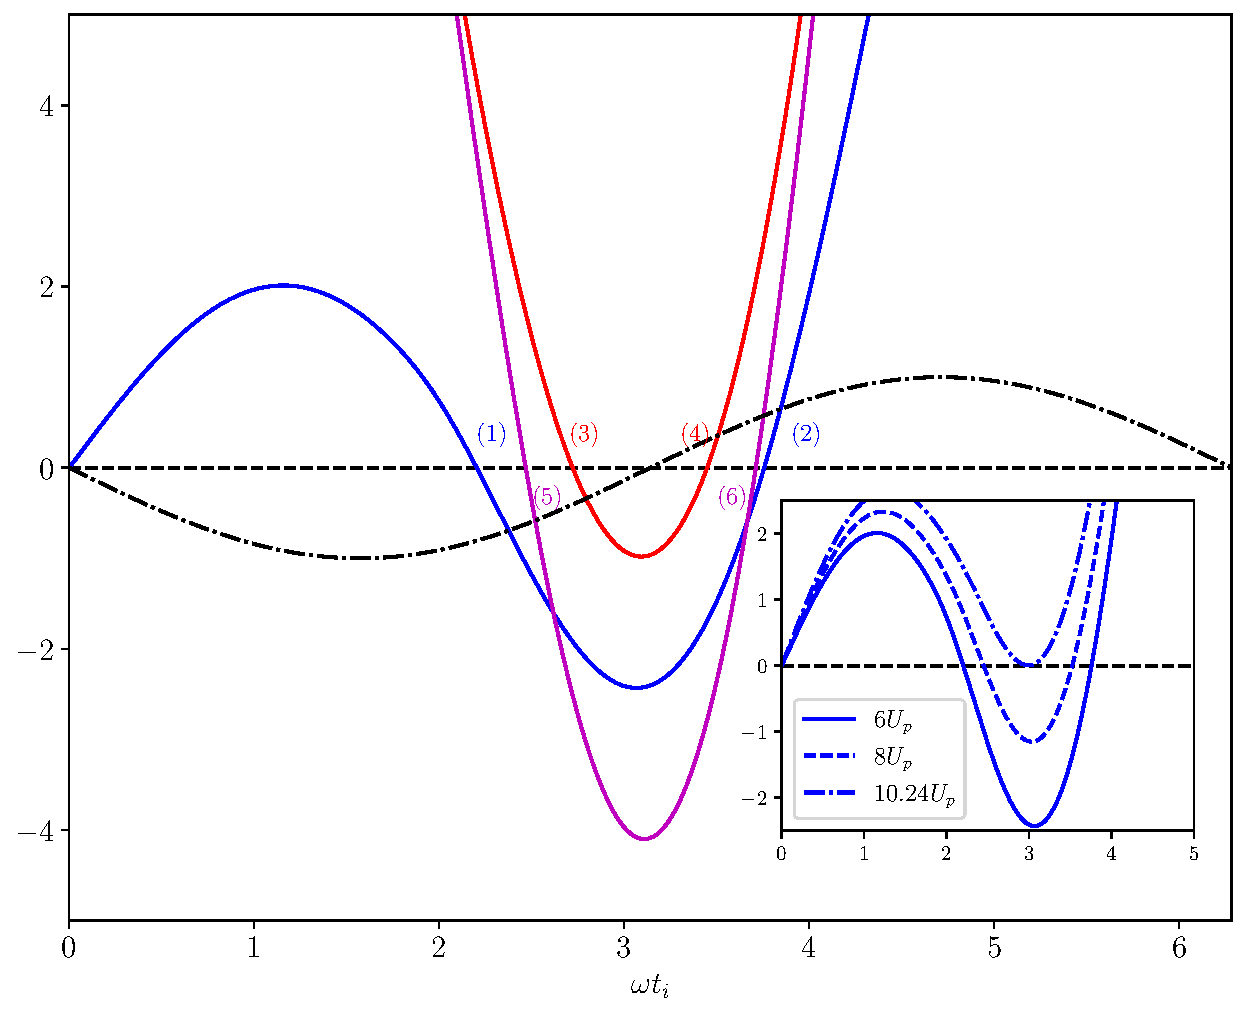
\includegraphics[width=\textwidth]{figures/ch_ATI_SPA/rescattering/return1to6inset.pdf}
  \end{subfigure}
  \begin{subfigure}[b]{0.55\linewidth}
    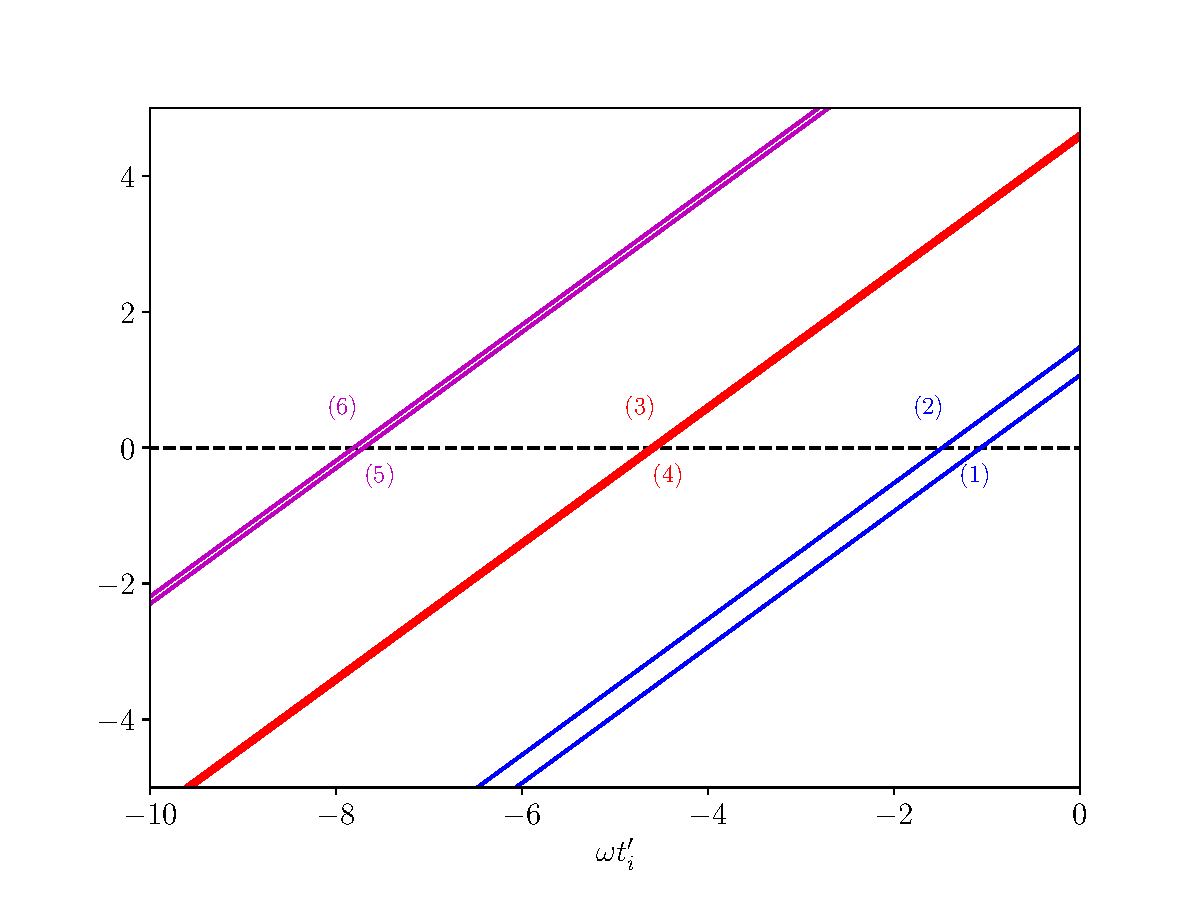
\includegraphics[width=\textwidth]{figures/ch_ATI_SPA/rescattering/release1to6.pdf}
  \end{subfigure}
  \caption{Results of a numerical determination of the return time
    $t_{i}$ and the release time $t'_{i}$ based on
    Eqs.~(\ref{eq:return_t}) and~(\ref{eq:release_t}) for a specified
    electron energy, $E_{p} = 6U_{p}$. The intersections with the $y =
    0$ axes indicate the real components of pairs of return time
    (left) and their corresponding release times (right). The numbers
    in parentheses refer to the numbers of individual
    trajectories. The electric field corresponding to the
    monochromatic field~(\ref{eq:lp_field}) is depicted in the left
    panel in dash-dotted lines. The inset in the left panel depicts
    the numerical solutions for the return time as the electron energy
    increases.}
  \label{fig:orbit_pairs}
\end{figure}


The complex orbits for the ionization time, rescattering time and
complex momentum, given by the saddle-point solutions of
Eqs.~(\ref{eq:return_t}) and~(\ref{eq:release_t}), are shown in
Figure~\ref{fig:complex_paths} for trajectories $i = (1,\dots,6)$ as a
function of the electron kinetic energy $E_{p}$. A subset of the
energy values is indicated in multiples of $U_{p}$ along the paths. In
the process of obtaining the saddle points corresponding to
trajectories with increasing travel times, the substitution $\omega t
\to \omega t + 2\pi k$, with $k = 0,1,\dots$, was implemented in
Eqs.~(\ref{eq:return_t}) and~(\ref{eq:release_t}). The behaviour of
these complex trajectories is markedly different depending on the
location of the classical cutoff. Every pair of trajectories shows
that the quantum orbits approach each other closely near the
cutoff. For energies above the cutoff, the orbits in every pair
diverge away from one another and the ones with negative imaginary
parts stop contributing to the \textsc{ati} spectrum and are dropped
from the sum~(\ref{eq:Mp_final}), as they lead to a diverging solution
for the probability amplitude. This cutoff marks a turning point in
the complex paths. It can be noticed that both the rescattering times
and quantum momenta have very small imaginary parts before the cutoff,
while their imaginary components become noticeable as the electron
energies increase beyond the cutoff. In contrast, the imaginary parts
of the ionization times are significant, indicating the origin of the
electrons through tunneling ionization. For energies above the cutoff,
the real components of the complex paths remain approximately constant
with increasing energy. As a result, a marked drop appears after the
cutoff in the spectrum associated with a given pair of trajectories.

% plot of saddle points
\begin{figure}
\begin{subfigure}[b]{0.33\linewidth}
  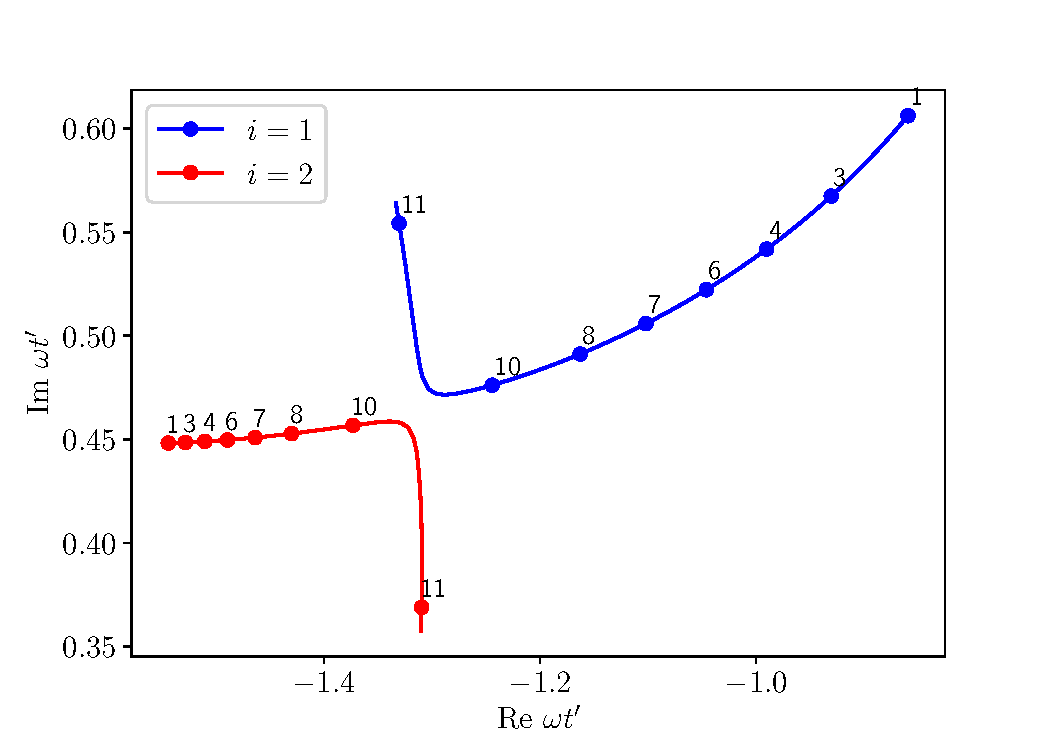
\includegraphics[width=\textwidth]{figures/ch_ATI_SPA/rescattering/start12.pdf}
\end{subfigure}
\begin{subfigure}[b]{0.33\linewidth}
  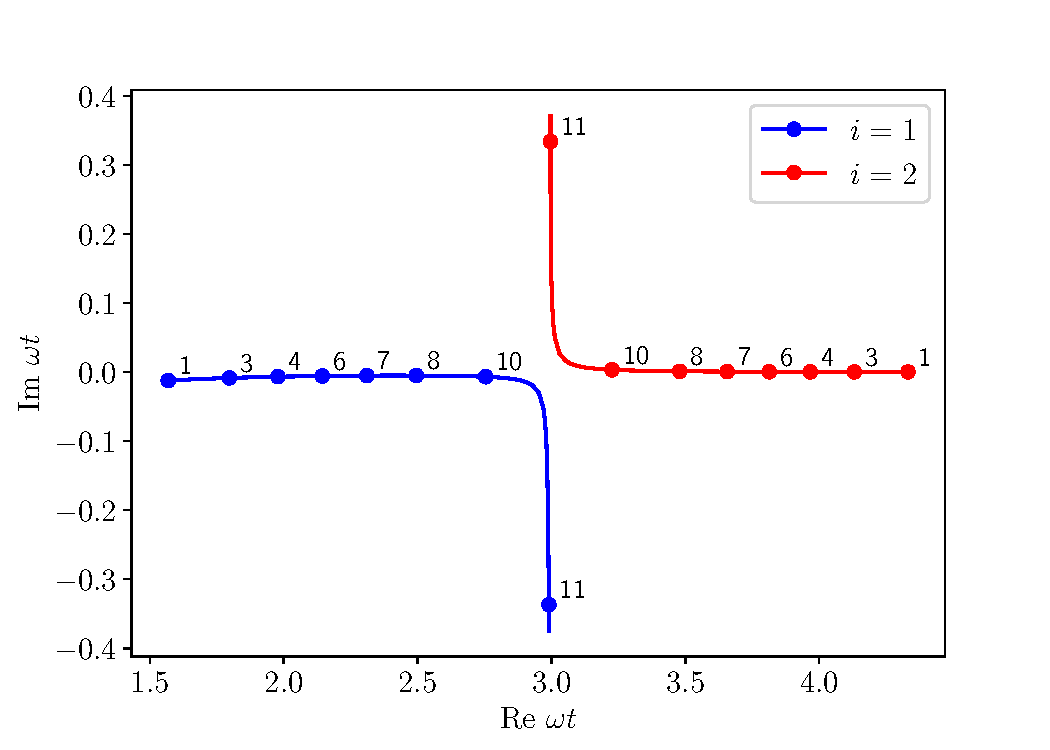
\includegraphics[width=\textwidth]{figures/ch_ATI_SPA/rescattering/return12.pdf}
\end{subfigure}
\begin{subfigure}[b]{0.33\linewidth}
  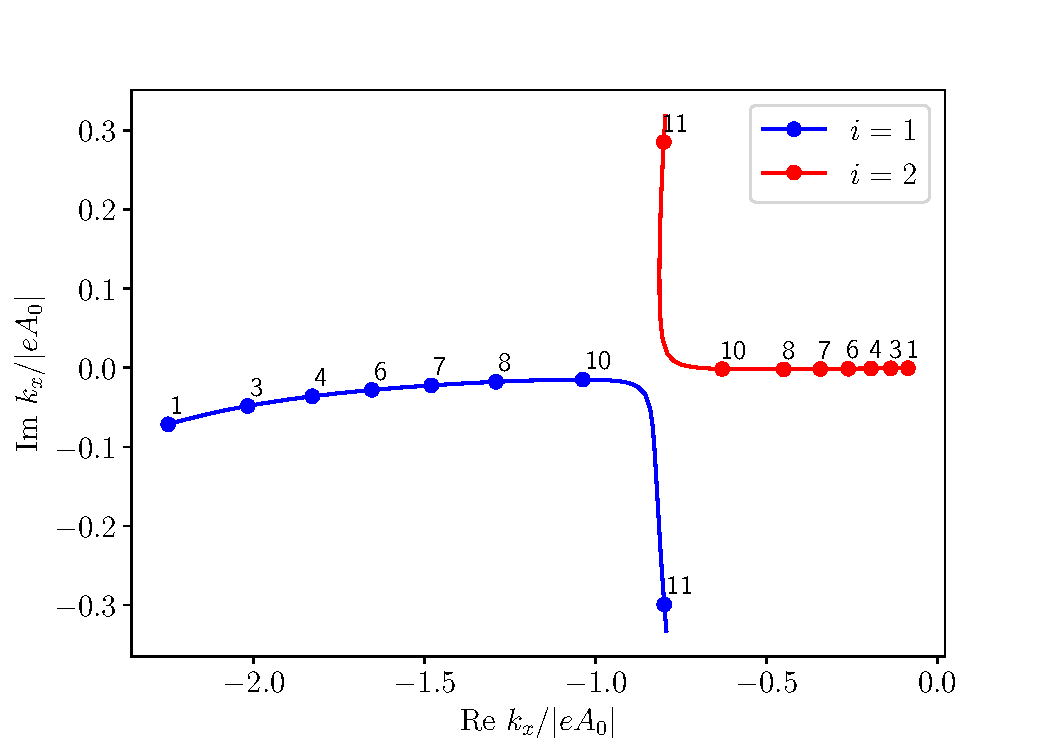
\includegraphics[width=\textwidth]{figures/ch_ATI_SPA/rescattering/momentum12.pdf}
\end{subfigure}
\begin{subfigure}[b]{0.33\linewidth}
  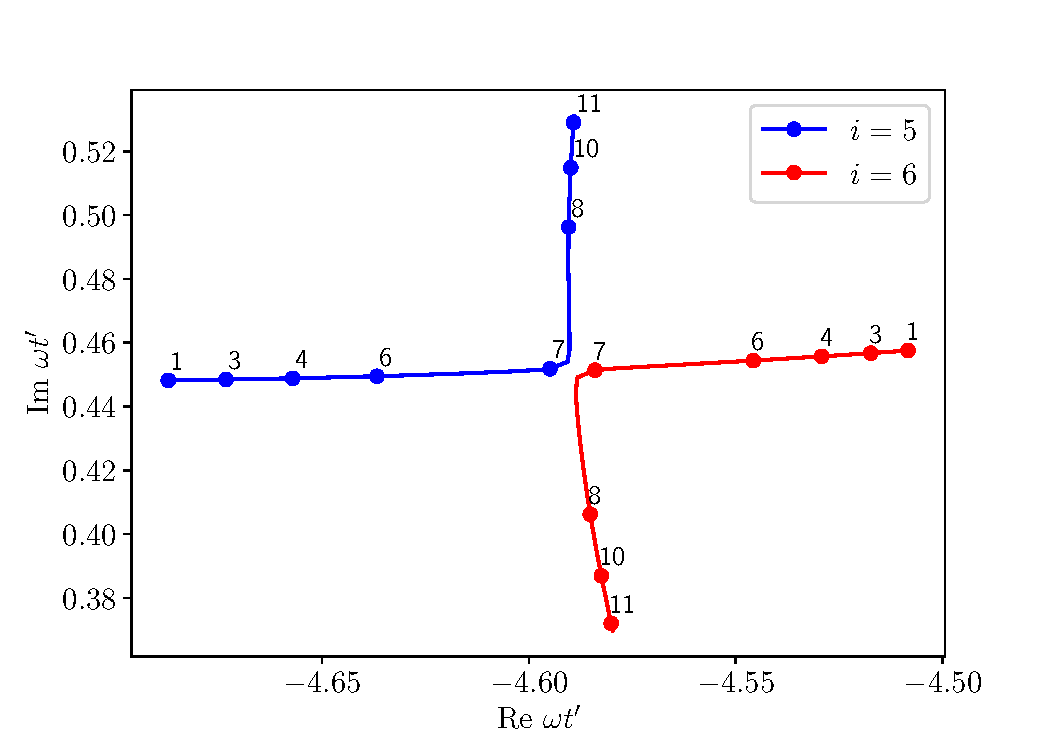
\includegraphics[width=\textwidth]{figures/ch_ATI_SPA/rescattering/start34.pdf}
\end{subfigure}
\begin{subfigure}[b]{0.33\linewidth}
  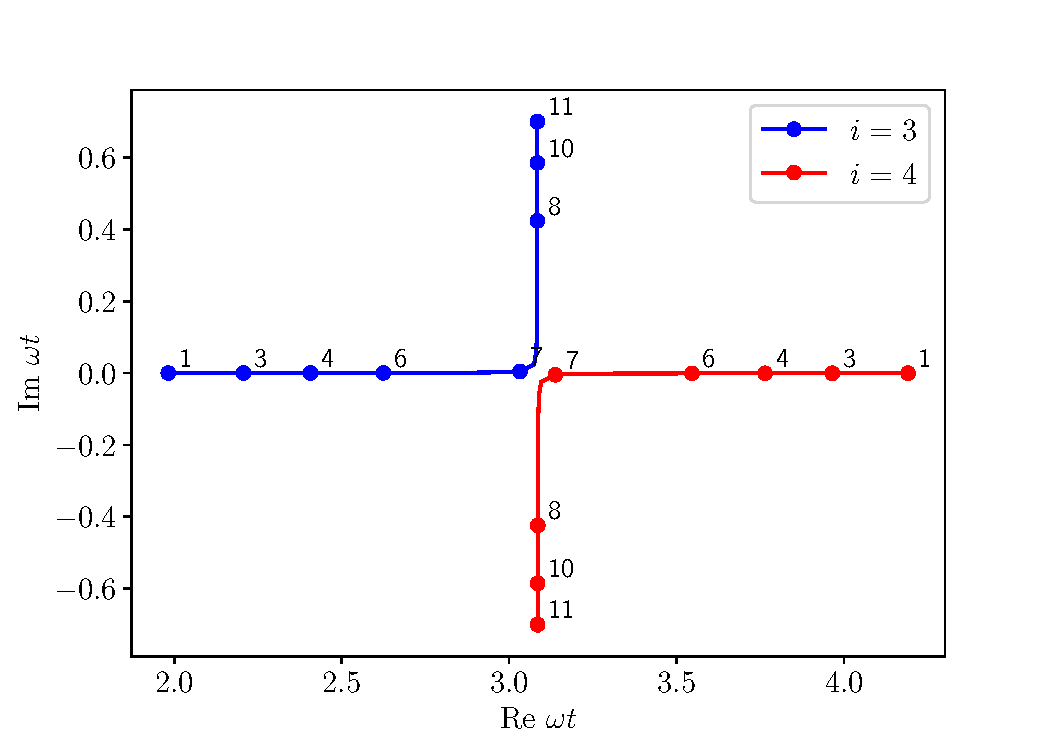
\includegraphics[width=\textwidth]{figures/ch_ATI_SPA/rescattering/return34.pdf}
\end{subfigure}
\begin{subfigure}[b]{0.33\linewidth}
  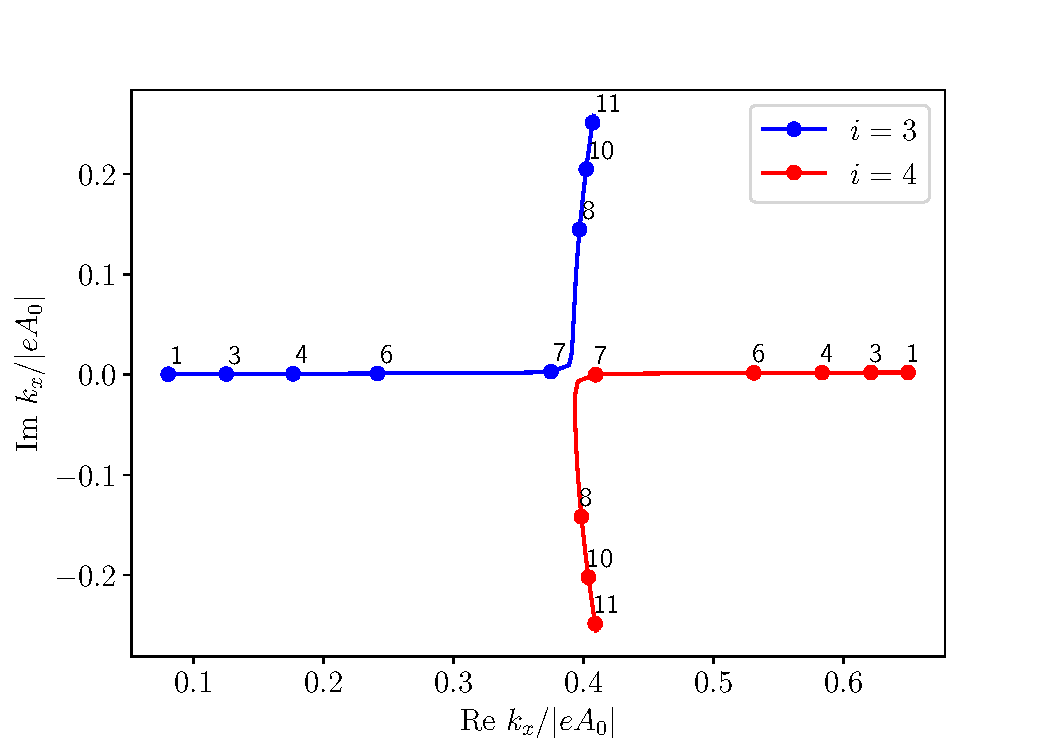
\includegraphics[width=\textwidth]{figures/ch_ATI_SPA/rescattering/momentum34.pdf}
\end{subfigure}
\begin{subfigure}[b]{0.33\linewidth}
  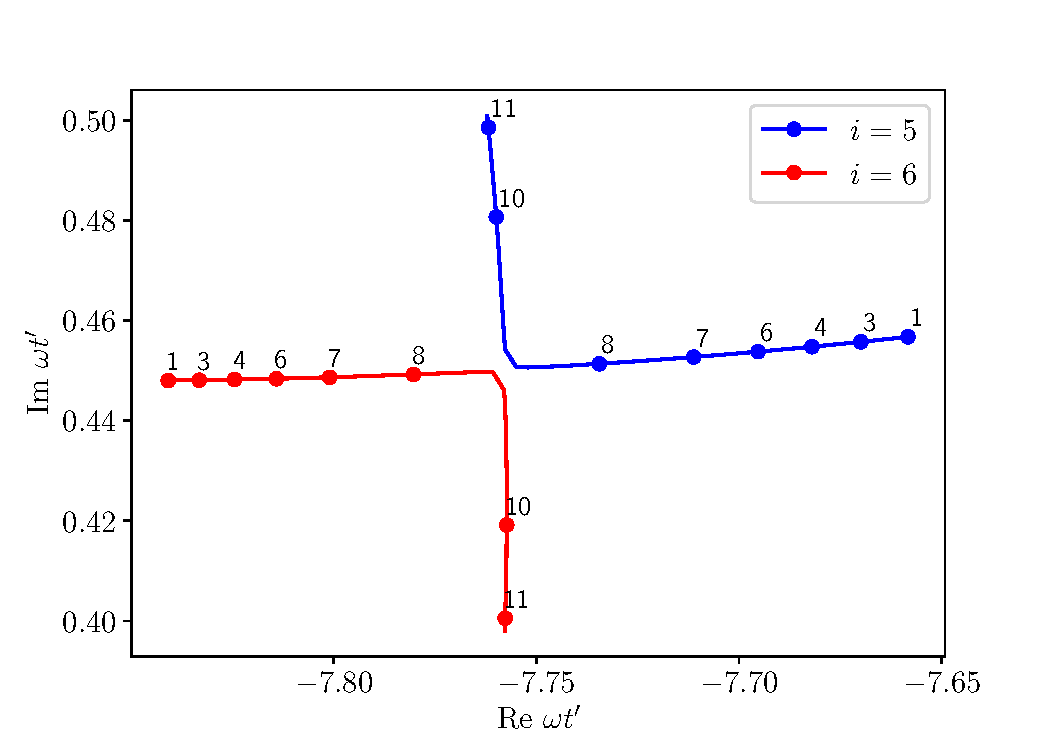
\includegraphics[width=\textwidth]{figures/ch_ATI_SPA/rescattering/start56.pdf}
\end{subfigure}
\begin{subfigure}[b]{0.33\linewidth}
  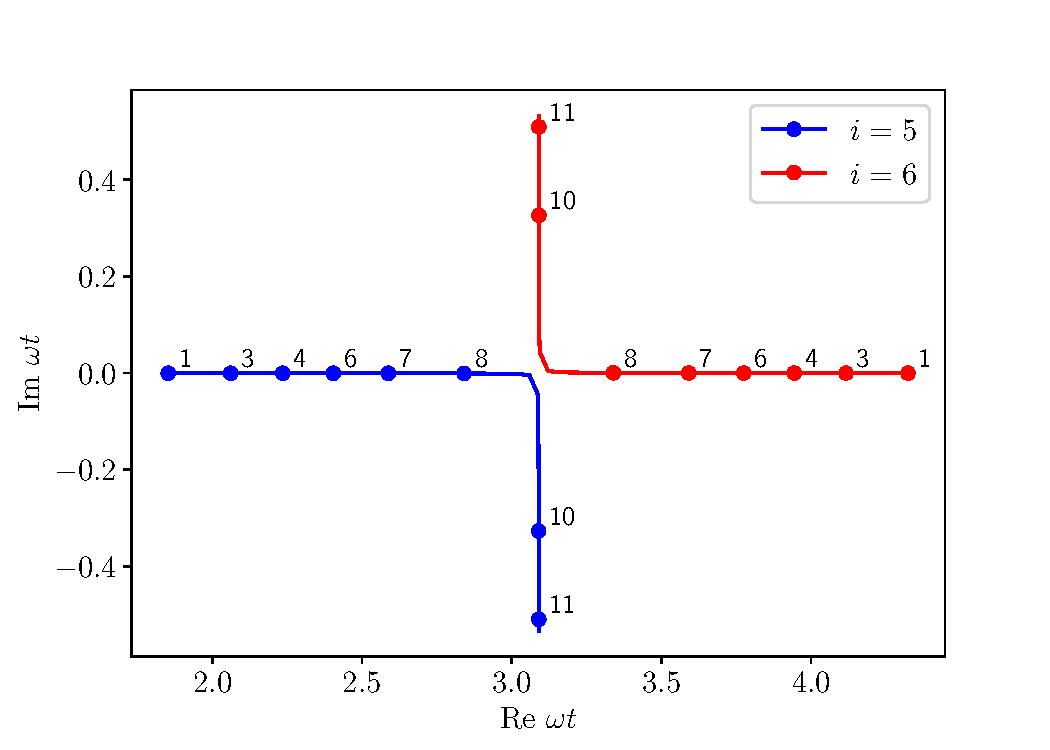
\includegraphics[width=\textwidth]{figures/ch_ATI_SPA/rescattering/return56.pdf}
\end{subfigure}
\begin{subfigure}[b]{0.33\linewidth}
  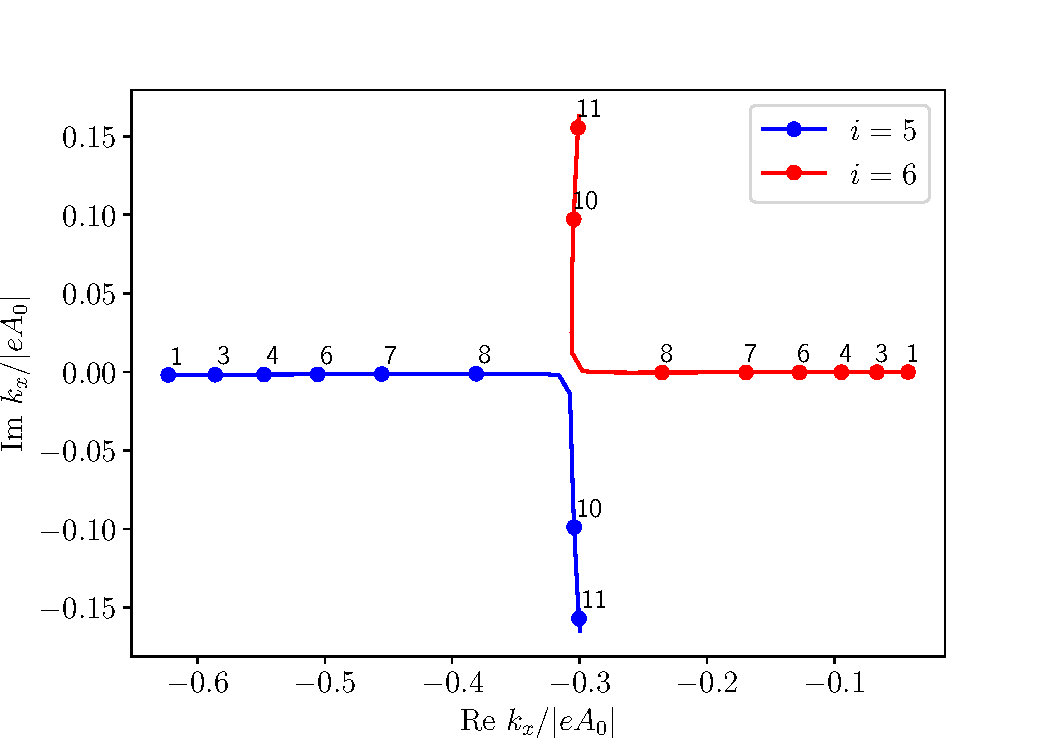
\includegraphics[width=\textwidth]{figures/ch_ATI_SPA/rescattering/momentum56.pdf}
\end{subfigure}
\caption{Saddle points for the orbits $(s = 1,\dots,6)$ in the complex
  plane as a function of the electron energy $E_{p}$ specified along
  the lines in multiples of $U_{p}$. A laser field of
  $10^{15}\ \mathrm{W/cm^{2}}$ and $\hbar\omega = 1.58\ \mathrm{eV}$
  and a binding energy of $E_{0} = -0.9\ \mathrm{a.u.}$ were used in
  the calculations. In this figure, $\omega t'$ represents the
  ionization time, $\omega t$ stands for rescattering time, and
  $k_{x}$ is the $x-$component of the canonical momentum
  $\mathbf{k}$. The underlying Keldysh parameter was set to $\gamma =
  0.464$.}
  \label{fig:complex_paths}
\end{figure}

% add algebra on the action for trajectories with rescattering and
% break down into real and imaginary components (based on the electron
% paths being complex to account for tunneling ionization), which is
% later shown in Fig. 5.5
It is illustrating to take into account the complex nature of the
electron dynamics in order to visualize how the action of the system,
$S(t_{i},t'_{i},\mathbf{k}_{i})$, evolves as the electron energy
increases. To this end, one can write the explicit analytic expression
for the action in the event that the canonical momentum $\mathbf{k}$
and the final momentum $\mathbf{p}$ are parallel to the linearly
polarized laser field~(\ref{eq:lp_field}), which reads
%
\begin{eqnarray}
  \label{eq:action_analytic}
S(t, t', \bf{k}) & = &
-\frac{1}{2} \int_{t}^{\infty} d\tau\left[ p^{2}
- 2eA_{0}p\cos(\omega\tau) + (eA_{0})^{2}\cos(\omega\tau)^{2} \right]\nonumber\\
&& -\frac{1}{2} \int_{t'}^{t} d\tau\left[k^{2}
- 2eA_{0}k\cos(\omega\tau) + (eA_{0})^{2}\cos(\omega\tau)^{2} \right]\nonumber\\
&& + \int_{-\infty}^{t'} d\tau|E_{0}|.
\end{eqnarray}
%
In the vicinity of the saddle points $(t_{i},t'_{i},\mathbf{k}_{i})$,
where the action satisfies the stationarity
condition~(\ref{eq:S_stationary}), the integration limits that cause
the integrand to diverge to $\pm\infty$ can be neglected. Some
algebraic simplifications on the analytic expression for the action
allow us to express the phase, $\Phi = (1/\eta)S$, in the probability
amplitude~(\ref{eq:Mp_final}) as
%
\begin{eqnarray}
  \label{eq:phase_final}
\Phi(t, t', \bf{k}) & = &
\left(\frac{E_{P}}{U_{P}} - \frac{k^{2}}{2U_{P}}\right) \omega t
+ \frac{2e}{\sqrt{U_{P}}} \left( k - \sqrt{2E_{P}}\right) \sin(\omega t) \nonumber\\
&&
+ \left( \frac{k^{2}}{2U_{P}} + e^{2}+2\gamma^{2} \right)\omega t'
- \frac{2e}{\sqrt{U_{P}}} k\sin(\omega t') \nonumber\\
&&
+ \frac{e^2}{2}\sin(2\omega t'),
\end{eqnarray}
%
where $E_{P} = p^{2}/2m$ indicates the electron energy.

%The phase is defined as Φ = (1/η)S = (ω/UP )S, where UP is the
%ponderomotive energy of the electron. Multiplying the action (12) by
%the 1/η factor and making use of the definitions of the ponderomotive
%energy and the Keldysh parameter one arrives at the expression


The actions $S(t_{i},t'_{i},\mathbf{k}_{i})/\eta$, with $\eta = 35.8$,
corresponding to the electron trajectories with the shortests travel
times $(i = 1, 2)$, are shown in Figure~\ref{fig:phase_ReIm} as a
function of the electron energy $E_{p}$ as blue/red lines,
respectively. A subset of energy values is specified along the curves
up to the cutoff energy, whereupon a crossing takes place between the
paths. Additionally, the complex coordinates of the action that were
graphically extracted from~\cite{phd_Kopold} are marked by crosses
($\times$) for the electron energies specified. The relative error
between the action~(\ref{eq:action_analytic}) and the saddle-point
results from~\cite{phd_Kopold} is indicated with errorbars for the
three energies considered. For energies below the cutoff the most
noticeable changes occur in the real components, while the imaginary
parts of the individual trajectories change little as they approach
each other along the plateau. In contrast to the saddle point
behaviour (Figure~\ref{fig:complex_paths}), where in a given pair of
trajectories $(i, j)$ they diverge rapidly from one another towards
the cutoff, the complex contributions of the action become more
similar as the electron energy increases and eventually are
interchanged at the cutoff, at which point one of the trajectories
ceases to contribute to the \textsc{ati} spectrum.
% MENTION THIS IN THE DESCRIPTION OF THE ATI SPECTRUM FIGURE
% Towards the cutoff, however, the trajectories and their
% contributions become more and more similar. Because of this, the
% last constructive interference at the cutoff is always most
% pronounced. Finally, the weights are interchanged and only one of
% the two trajectories may continue to be taken into account

% plot of action in phase-space
\begin{figure}
  \centering 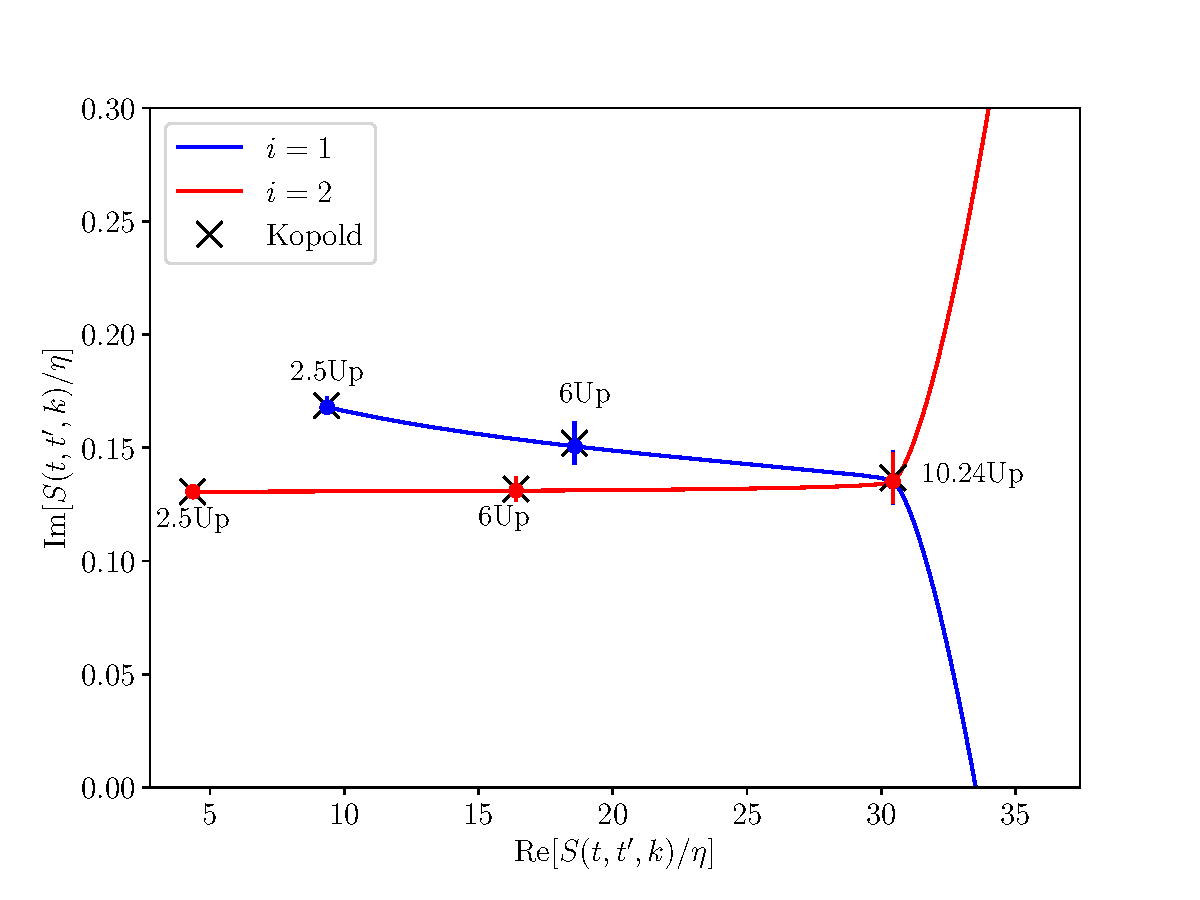
\includegraphics[width =
    0.75\textwidth]{figures/ch_ATI_SPA/rescattering/phase_ComplexReIm.pdf}
  \caption{Representation of the action in the complex plane for the
    two shortest trajectories $(1, 2)$ shown in blue and red
    respectively. In addition, the complex coordinates for the action
    extracted from~\cite{phd_Kopold} are shown as $\times$ for the
    specified energy values.}
  \label{fig:phase_ReIm}
\end{figure}

% mention errorbars in the plot of the action in the complex plane for
% paths 1 and 2

The computation of the \textsc{ati} spectrum can now be carried out
once the solutions of the saddle-point equations are determined. To
this end, the appropriate subset of electron trajectories is inserted
into the matrix element~(\ref{eq:Mp_final}).

\begin{figure}
  \centering 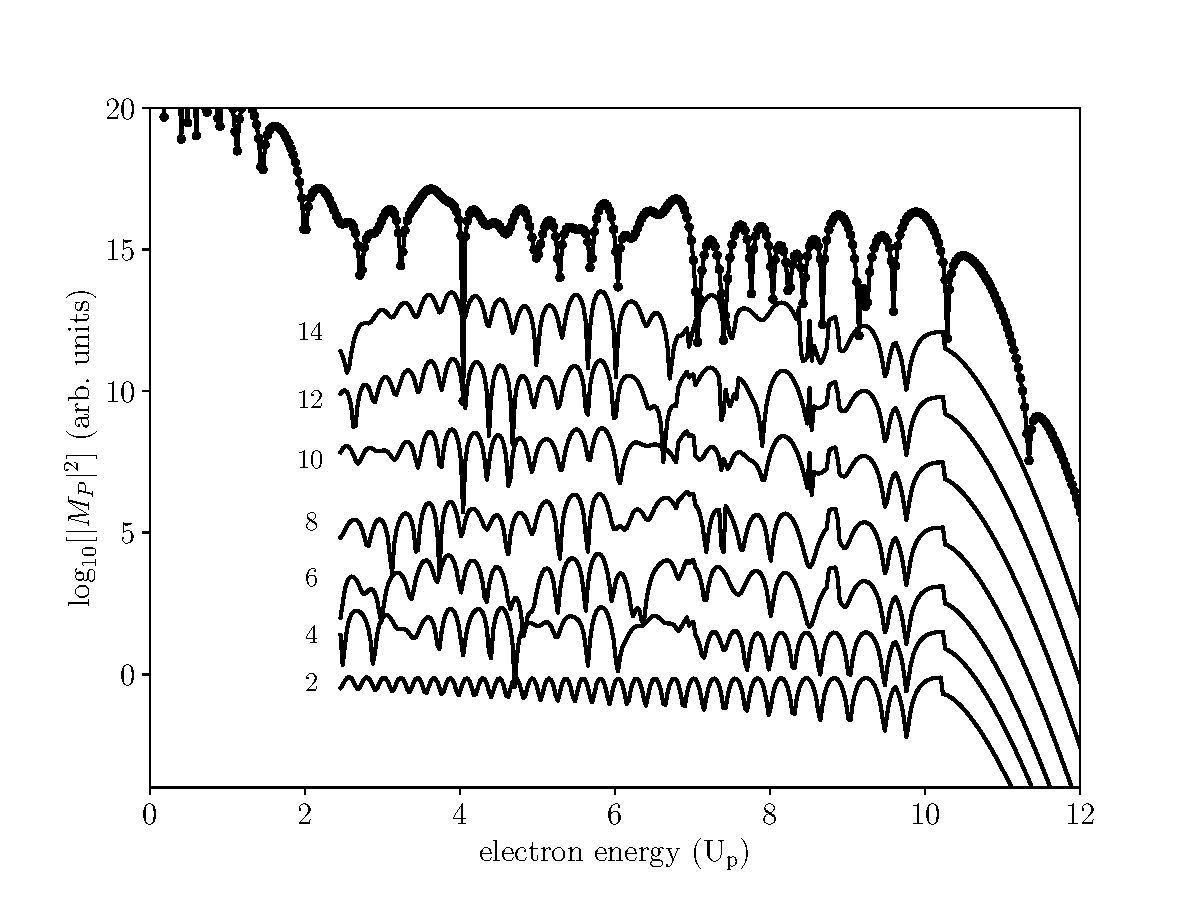
\includegraphics[width =
    0.75\textwidth]{figures/ch_ATI_SPA/rescattering/14pathsvsqm.pdf}
  \caption{Saddle-point evaluation of the \textsc{ati} spectrum as a
    function of the electron energy in terms of an increasing number
    of quantum paths. A laser intensity of
    $10^{15}\ \mathrm{W/cm^{2}}$ and frequency $\hbar\omega =
    0.0584\ \mathrm{a.u.}$ were used in the calculations, as well as a
    binding energy of $E_{0} = -0.9\ \mathrm{a.u.}$ corresponding to a
    model-helium atom.}
  \label{fig:ati_spectrum}
\end{figure}


% plot of formation of the spectrum as the number of trajectories
% increases






%%% Local Variables:
%%% mode: latex
%%% TeX-master: "thesis"
%%% End:
